\documentclass[10pt]{article}

\usepackage[margin=0.58in]{geometry}
\usepackage{xcolor}
\usepackage{tikz}
\usetikzlibrary{arrows.meta,positioning,shapes.geometric,fit,backgrounds,calc}
\usepackage[most]{tcolorbox}
\usepackage{listings}
\usepackage{pdflscape}
\usepackage{booktabs}
\usepackage{fancyhdr}
\usepackage{titlesec}
\usepackage{hyperref}

\definecolor{violet}{HTML}{5E17EB}
\definecolor{lightviolet}{HTML}{8755F5}
\definecolor{lavender}{HTML}{EEE7FF}
\definecolor{softlavender}{HTML}{F8F5FF}
\definecolor{mint}{HTML}{20C997}
\definecolor{warmyellow}{HTML}{FFC857}
\definecolor{darktext}{HTML}{191522}
\definecolor{secondarytext}{HTML}{777180}
\definecolor{bordergray}{HTML}{EAE7F0}
\definecolor{warningtext}{HTML}{A66B00}
\definecolor{warningbg}{HTML}{FFF8E1}

\hypersetup{colorlinks=true,linkcolor=violet,urlcolor=violet,pdftitle={ReDeal - System Architecture and Demo Status}}

\pagestyle{fancy}
\fancyhf{}
\lhead{\textcolor{violet}{ReDeal}}
\rhead{\textcolor{secondarytext}{System Architecture}}
\cfoot{\thepage}

\titleformat{\section}{\large\bfseries\color{violet}}{\thesection}{0.5em}{}
\titlespacing*{\section}{0pt}{8pt}{4pt}
\setlength{\parindent}{0pt}
\setlength{\parskip}{4pt}

\newcommand{\code}[1]{\texttt{#1}}
\newcommand{\demo}{\textcolor{mint}{\textbf{DEMO}}}
\newcommand{\prototype}{\textcolor{warningtext}{\textbf{PROTOTYPE}}}
\newcommand{\pending}{\textcolor{violet}{\textbf{PENDING}}}

\newtcolorbox{stagebox}{enhanced,breakable,colback=lavender,colframe=violet,title=Current Project Stage,fonttitle=\bfseries,coltitle=darktext,boxrule=0.8pt,arc=2mm}
\newtcolorbox{limitbox}{enhanced,breakable,colback=warningbg,colframe=warmyellow,title=Demo Limitations -- Please Read,fonttitle=\bfseries,coltitle=darktext,boxrule=1pt,arc=2mm}

\lstdefinelanguage{JavaScript}{
  keywords={const,let,var,function,return,if,else,for,while,async,await,import,from,export,class,new,true,false,null,undefined},
  sensitive=true,comment=[l]{//},morecomment=[s]{/*}{*/},morestring=[b]",morestring=[b]'
}
\lstset{language=JavaScript,basicstyle=\ttfamily\scriptsize,keywordstyle=\color{violet}\bfseries,commentstyle=\color{secondarytext},stringstyle=\color{warningtext},frame=single,rulecolor=\color{bordergray},backgroundcolor=\color{softlavender},breaklines=true,showstringspaces=false,columns=fullflexible}

\begin{document}

\begin{center}
  {\Huge\bfseries\color{violet} ReDeal -- Second-Hand Marketplace}\\[3pt]
  {\large\color{secondarytext} System Architecture and Demo Status}\\[8pt]
  {\small Date: November 5, 2026 \quad\textbullet\quad Current HEAD: \code{5efe2dd} \quad\textbullet\quad Working tree: clean}
\end{center}

\section{Current Stage}
\begin{stagebox}
\textbf{Phases 0--3:} CLOSED. Phase 2 and Phase 3 close-out records include browser verification; earlier historical entries contain intermediate unverified statuses.

\textbf{Phase 4 -- Authentication:} Implemented and source-audited with conditions. Browser verification is pending.

\textbf{Planned next work:} Profile completion and listing CRUD, Request System, search and filter enhancements, accessibility QA, and TeleportHQ directory cleanup.

\textbf{Intended use:} Classroom demonstration and academic prototype.
\end{stagebox}

\section{Executive Summary}
ReDeal is a Philippine second-hand marketplace prototype for browsing, favoriting, and creating listings. Product prices use Philippine Peso formatting, the interface follows the Electric Violet design system, and the application is implemented with semantic HTML5, CSS3, and native JavaScript ES modules.

The application uses local mock data and browser \code{localStorage}. There is no backend, database, framework, build step, or real authentication service. The current source supports marketplace browsing, client-side search/filter/sort, product detail pages, favorites, listing creation, login/signup flows, session persistence, a profile page, and prototype messaging/offer dialogs.

\begin{lstlisting}
login.html -> Login.js -> auth.js -> localStorage
marketplace.html -> Marketplace.js -> products.js
create-listing.html -> CreateListing.js -> storage.js
profile.html -> Profile.js -> auth.js + favorites.js
\end{lstlisting}

\begin{tcolorbox}[colback=softlavender,colframe=bordergray,title=Repository Map,fonttitle=\bfseries,coltitle=darktext,boxrule=0.5pt]
\small
\textbf{Root HTML:} \code{index.html}, \code{marketplace.html}, \code{product.html}, \code{create-listing.html}, \code{login.html}, \code{signup.html}, \code{profile.html}, \code{messages.html}, \code{requests.html}, \code{sell.html}.\\
\textbf{CSS:} \code{variables.css}, \code{main.css}, \code{components.css}, \code{create-listing.css}, \code{product-detail.css}, \code{login.css}, \code{signup.css}, \code{profile.css}. \code{layout.css} is not present.\\
\textbf{Data:} \code{products.js}, \code{categories.js}, \code{storage.js}, \code{auth.js}.\\
\textbf{Pages:} \code{ProductDetail.js}, \code{Marketplace.js}, \code{CreateListing.js}, \code{Login.js}, \code{Signup.js}, \code{Profile.js}, \code{Messages.js}, \code{Requests.js}.\\
\textbf{Components:} \code{Card.js}, \code{Modal.js}, \code{Header.js}, \code{UserMenu.js}.\\
\textbf{Utilities:} \code{dom.js}, \code{favorites.js}, \code{auth-guard.js}, \code{events.js}.
\end{tcolorbox}

\clearpage
\begin{landscape}
\section{System Architecture Diagram}
\begin{center}
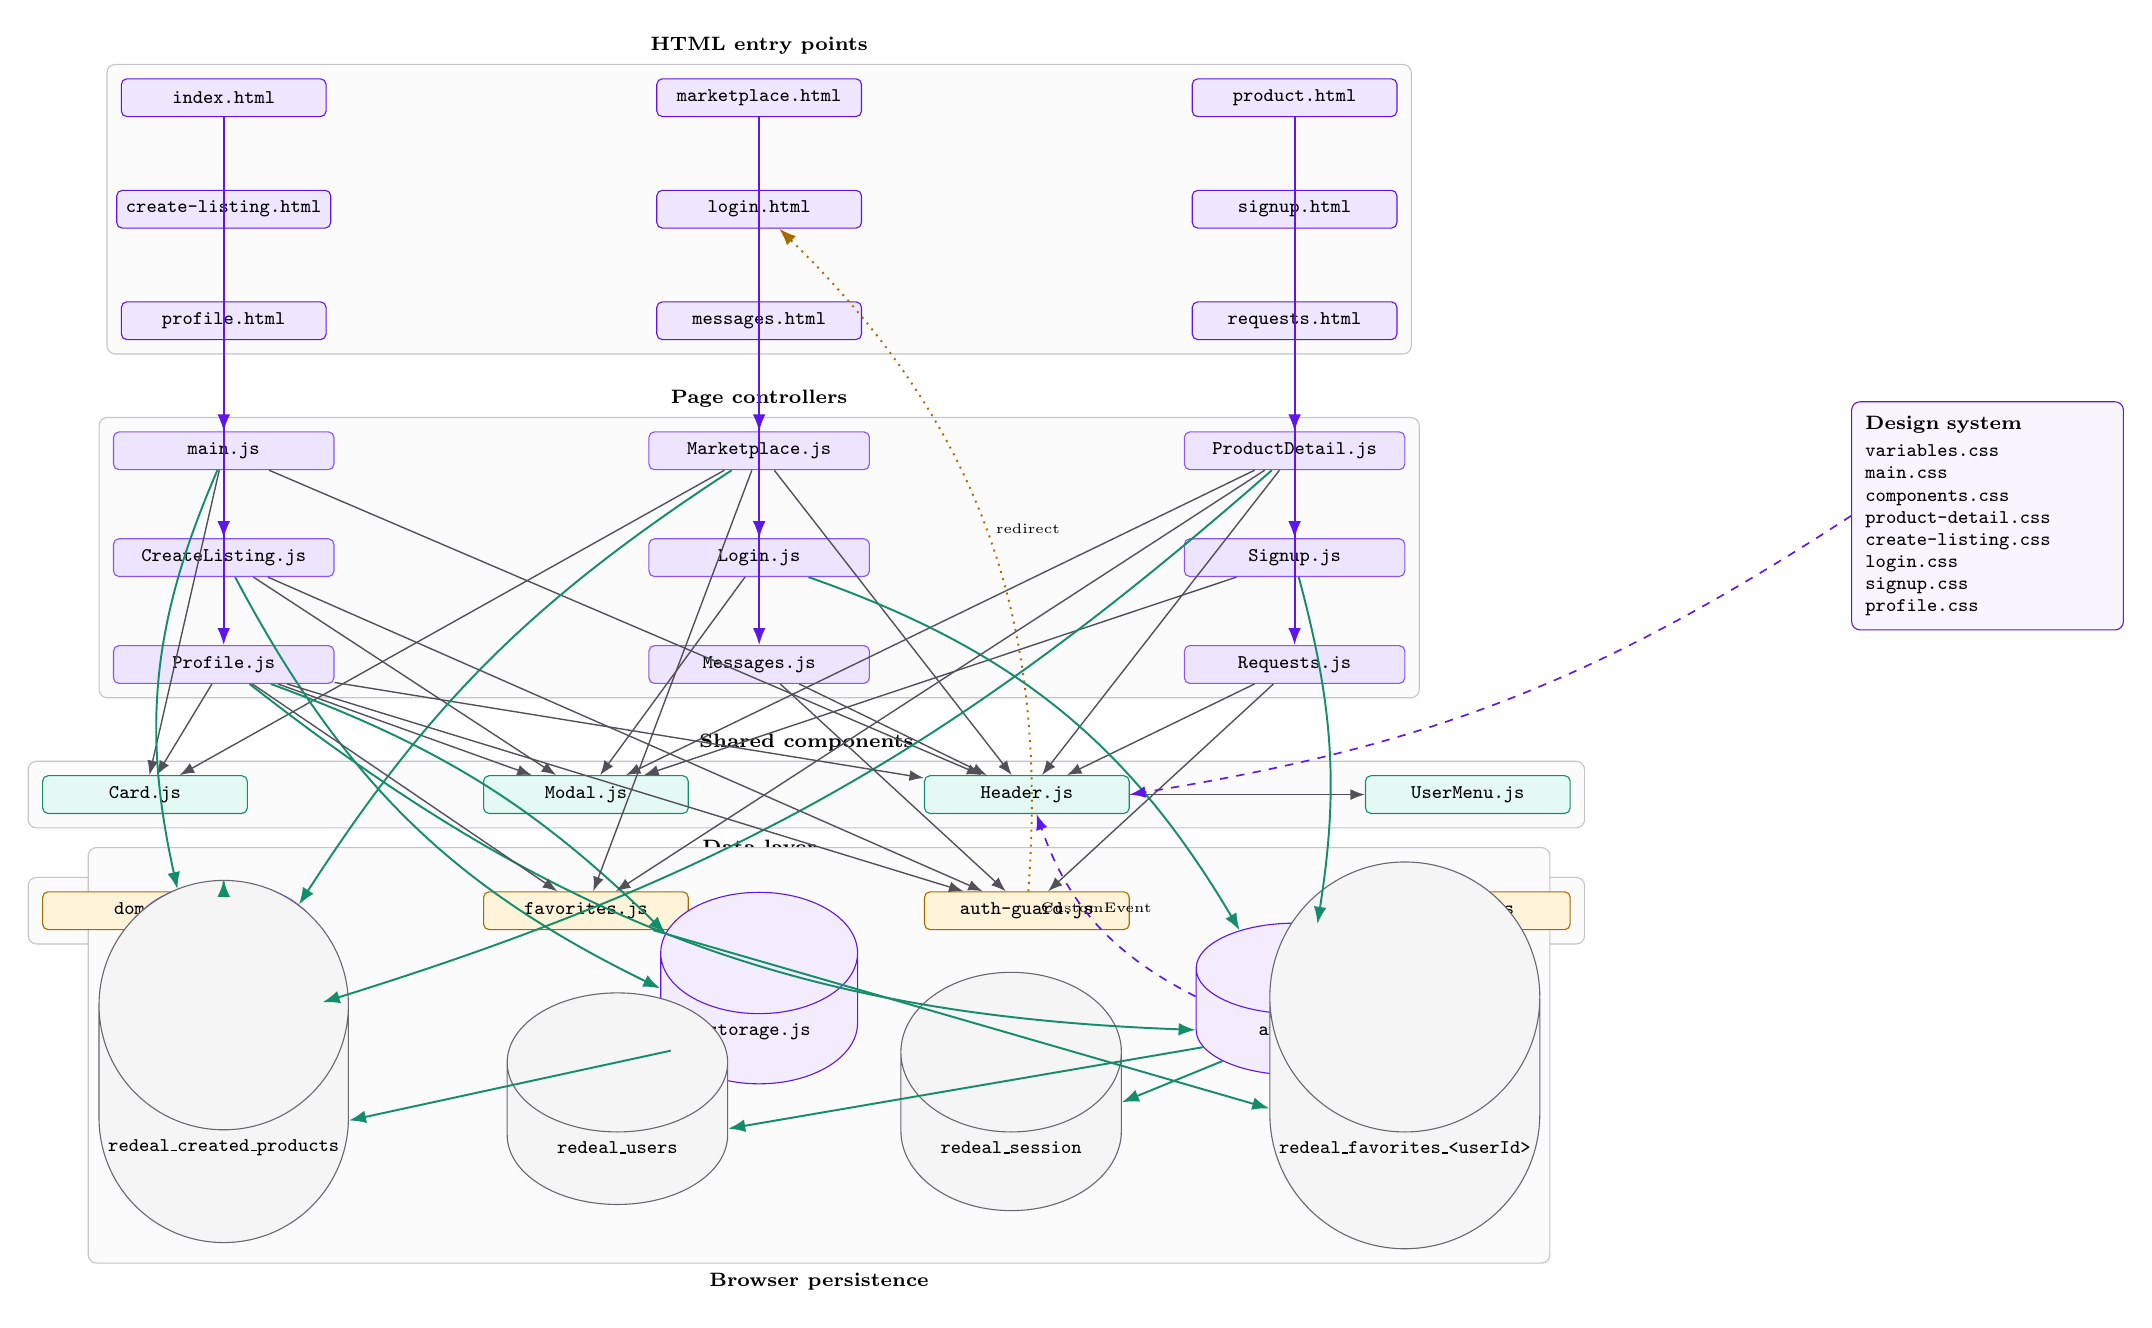
\begin{tikzpicture}[
  x=2cm,y=1.18cm,transform shape,
  page/.style={rectangle,rounded corners=2pt,draw=violet,fill=lavender,minimum width=2.6cm,minimum height=0.48cm,align=center,font=\scriptsize},
  controller/.style={rectangle,rounded corners=2pt,draw=lightviolet,fill=lightviolet!15,minimum width=2.8cm,minimum height=0.48cm,align=center,font=\scriptsize},
  component/.style={rectangle,rounded corners=2pt,draw=mint!70!black,fill=mint!12,minimum width=2.6cm,minimum height=0.48cm,align=center,font=\scriptsize},
  utility/.style={rectangle,rounded corners=2pt,draw=warningtext,fill=warmyellow!22,minimum width=2.6cm,minimum height=0.48cm,align=center,font=\scriptsize},
  data/.style={cylinder,shape border rotate=90,draw=violet,fill=violet!8,minimum width=2.5cm,minimum height=0.65cm,align=center,font=\scriptsize},
  store/.style={cylinder,shape border rotate=90,draw=darktext!65,fill=gray!8,minimum width=2.8cm,minimum height=0.6cm,align=center,font=\scriptsize},
  design/.style={rectangle,rounded corners=3pt,draw=violet,fill=softlavender,text width=3.1cm,minimum height=2.4cm,align=left,font=\scriptsize,inner sep=5pt},
  layer/.style={rounded corners=3pt,draw=darktext!25,fill=gray!3,inner sep=5pt},
  load/.style={-Latex,draw=violet,line width=0.7pt},
  uses/.style={-Latex,draw=darktext!75,line width=0.5pt},
  dataflow/.style={-Latex,draw=mint!70!black,line width=0.7pt},
  event/.style={-Latex,draw=violet,dashed,line width=0.6pt},
  redirect/.style={-Latex,draw=warningtext,dotted,line width=0.7pt}
]

\node[page] (pindex) at (0,11.3) {\code{index.html}};
\node[page] (pmarket) at (3.4,11.3) {\code{marketplace.html}};
\node[page] (pproduct) at (6.8,11.3) {\code{product.html}};
\node[page] (pcreate) at (0,10.1) {\code{create-listing.html}};
\node[page] (plogin) at (3.4,10.1) {\code{login.html}};
\node[page] (psignup) at (6.8,10.1) {\code{signup.html}};
\node[page] (pprofile) at (0,8.9) {\code{profile.html}};
\node[page] (pmessages) at (3.4,8.9) {\code{messages.html}};
\node[page] (prequests) at (6.8,8.9) {\code{requests.html}};

\node[controller] (cmain) at (0,7.5) {\code{main.js}};
\node[controller] (cmarket) at (3.4,7.5) {\code{Marketplace.js}};
\node[controller] (cproduct) at (6.8,7.5) {\code{ProductDetail.js}};
\node[controller] (ccreate) at (0,6.35) {\code{CreateListing.js}};
\node[controller] (clogin) at (3.4,6.35) {\code{Login.js}};
\node[controller] (csignup) at (6.8,6.35) {\code{Signup.js}};
\node[controller] (cprofile) at (0,5.2) {\code{Profile.js}};
\node[controller] (cmessages) at (3.4,5.2) {\code{Messages.js}};
\node[controller] (crequests) at (6.8,5.2) {\code{Requests.js}};

\node[component] (card) at (-0.5,3.8) {\code{Card.js}};
\node[component] (modal) at (2.3,3.8) {\code{Modal.js}};
\node[component] (header) at (5.1,3.8) {\code{Header.js}};
\node[component] (menu) at (7.9,3.8) {\code{UserMenu.js}};

\node[utility] (dom) at (-0.5,2.55) {\code{dom.js}};
\node[utility] (favorites) at (2.3,2.55) {\code{favorites.js}};
\node[utility] (guard) at (5.1,2.55) {\code{auth-guard.js}};
\node[utility] (events) at (7.9,2.55) {\code{events.js}};

\node[data] (products) at (0,1.25) {\code{products.js}};
\node[data] (storage) at (3.4,1.25) {\code{storage.js}};
\node[data] (auth) at (6.8,1.25) {\code{auth.js}};

\node[store] (created) at (0,0) {\code{redeal\_created\_products}};
\node[store] (users) at (2.5,0) {\code{redeal\_users}};
\node[store] (session) at (5,0) {\code{redeal\_session}};
\node[store] (favstore) at (7.5,0) {\code{redeal\_favorites\_<userId>}};

\node[design] (design) at (11.2,6.8) {
  \textbf{Design system}\\[2pt]
  \code{variables.css}\\
  \code{main.css}\\
  \code{components.css}\\
  \code{product-detail.css}\\
  \code{create-listing.css}\\
  \code{login.css}\\
  \code{signup.css}\\
  \code{profile.css}
};

\draw[load] (pindex)--(cmain); \draw[load] (pmarket)--(cmarket); \draw[load] (pproduct)--(cproduct);
\draw[load] (pcreate)--(ccreate); \draw[load] (plogin)--(clogin); \draw[load] (psignup)--(csignup);
\draw[load] (pprofile)--(cprofile); \draw[load] (pmessages)--(cmessages); \draw[load] (prequests)--(crequests);

\draw[uses] (cmain)--(card); \draw[uses] (cmain)--(header);
\draw[uses] (cmarket)--(card); \draw[uses] (cmarket)--(header);
\draw[uses] (cproduct)--(modal); \draw[uses] (cproduct)--(header);
\draw[uses] (ccreate)--(modal); \draw[uses] (cprofile)--(card); \draw[uses] (cprofile)--(modal); \draw[uses] (cprofile)--(header);
\draw[uses] (clogin)--(modal); \draw[uses] (csignup)--(modal); \draw[uses] (cmessages)--(header); \draw[uses] (crequests)--(header);
\draw[uses] (header)--(menu);

\draw[dataflow] (cmain) to[bend right=18] (products);
\draw[dataflow] (cmarket) to[bend right=12] (products);
\draw[dataflow] (cproduct) to[bend left=12] (products);
\draw[dataflow] (ccreate) to[bend right=18] (storage);
\draw[dataflow] (clogin) to[bend left=20] (auth);
\draw[dataflow] (csignup) to[bend left=12] (auth);
\draw[dataflow] (cprofile) to[bend right=18] (auth);
\draw[dataflow] (cprofile) to[bend left=12] (storage);

\draw[uses] (cproduct)--(favorites); \draw[uses] (cmarket)--(favorites); \draw[uses] (cprofile)--(favorites);
\draw[uses] (ccreate)--(guard); \draw[uses] (cprofile)--(guard); \draw[uses] (cmessages)--(guard); \draw[uses] (crequests)--(guard);

\draw[dataflow] (products)--(created); \draw[dataflow] (storage)--(created);
\draw[dataflow] (auth)--(users); \draw[dataflow] (auth)--(session); \draw[dataflow] (favorites)--(favstore);
\draw[event] (auth) to[bend left=22] node[above,font=\tiny] {CustomEvent} (header);
\draw[redirect] (guard) to[bend right=25] node[right,font=\tiny] {redirect} (plogin);
\draw[event] (design.west) to[bend left=12] (header.east);

\begin{pgfonlayer}{background}
  \node[layer,fit=(pindex)(prequests),label={[font=\scriptsize\bfseries]above:HTML entry points}] {};
  \node[layer,fit=(cmain)(crequests),label={[font=\scriptsize\bfseries]above:Page controllers}] {};
  \node[layer,fit=(card)(menu),label={[font=\scriptsize\bfseries]above:Shared components}] {};
  \node[layer,fit=(dom)(events),label={[font=\scriptsize\bfseries]above:Utilities}] {};
  \node[layer,fit=(products)(auth),label={[font=\scriptsize\bfseries]above:Data layer}] {};
  \node[layer,fit=(created)(favstore),label={[font=\scriptsize\bfseries]below:Browser persistence}] {};
\end{pgfonlayer}
\end{tikzpicture}
\end{center}

\begin{tcolorbox}[colback=softlavender,colframe=bordergray,boxrule=0.5pt,arc=1mm]
\scriptsize
\textbf{Legend:} rounded violet rectangles are HTML entry points; light-violet rectangles are page controllers; mint rectangles are shared components; yellow rectangles are utilities; cylinders are data or persistence; solid arrows indicate loading or use; green arrows indicate data flow; dashed arrows indicate events; dotted arrows indicate redirects.
\end{tcolorbox}
\end{landscape}

\clearpage
\section{What Works Today}
\begin{tabular}{@{}p{4.2cm}p{9.4cm}@{}}
\toprule
\textbf{Feature} & \textbf{Current source-backed status} \\
\midrule
Marketplace browsing & \demo\ 15 seed products with seller names, prices, local JPG images, categories, conditions, and locations. \\
Search, filters, and sorting & \demo\ Client-side query search, category filtering, condition filtering, sorting, URL state, and clear-filters behavior are implemented. \\
Product details & \demo\ Product lookup, seller information, description, condition, favorite controls, share fallback, and responsive action controls. The current model stores one image per product. \\
Favorites & \demo\ User-scoped localStorage keys, reload persistence, same-document event synchronization, and legacy-key migration. Cross-tab synchronization is not implemented. \\
Message Seller / Make Offer & \prototype\ Modal flows validate input and show confirmation alerts, but no message or offer is sent to a backend. \\
Create Listing & \demo\ Form validation, seller identity, image URL, localStorage persistence, generated ID, and redirect to the new product. \\
Authentication & \pending\ Login, signup, demo login, session restore, route guards, and logout exist in source. Browser verification is still required. \\
Header auth state & \pending\ Guest controls and authenticated avatar menu exist in source. Browser verification and final touch-target QA remain. \\
Profile page & \pending\ User information, own listings, favorites, statistics, settings, and logout exist in source. Browser verification remains open. \\
\bottomrule
\end{tabular}

\section{Demo Limitations -- Read First}
\begin{limitbox}
\small
\textbf{This is a front-end prototype for a classroom demonstration.}

\begin{minipage}[t]{0.48\linewidth}
\begin{enumerate}
  \setlength{\itemsep}{1pt}
  \item \textbf{No backend.} Data is stored in the browser. Clearing site storage removes local users, sessions, favorites, and created listings.
  \item \textbf{Passwords are not secure.} Passwords are stored in plaintext in \code{localStorage}; use fake credentials only.
  \item \textbf{No real accounts.} Sessions are local browser records and can be inspected or modified.
  \item \textbf{Messaging is simulated.} Message Seller and Make Offer only show prototype confirmation dialogs.
  \item \textbf{Requests are not implemented.} The Requests page is a protected placeholder.
  \item \textbf{Listing CRUD is incomplete.} Edit, delete, and archive actions are not implemented.
  \item \textbf{No server-side search.} Search and filters operate only on locally loaded mock data.
\end{enumerate}
\end{minipage}
\hfill
\begin{minipage}[t]{0.48\linewidth}
\begin{enumerate}
  \setlength{\itemsep}{1pt}
  \setcounter{enumi}{7}
  \item \textbf{Image input is URL-based.} Seed images are local JPGs; a new listing can reference a remote image URL.
  \item \textbf{Single image per product.} There is no multi-image upload or gallery model.
  \item \textbf{Favorites are not cross-tab synchronized.} The custom event is same-document; the \code{storage} event is not used.
  \item \textbf{No notifications.} There are no email, push, or in-app notification services.
  \item \textbf{No payments.} ReDeal is a listing interface, not a transaction processor.
  \item \textbf{No identity verification.} Email, phone, and government-ID verification are absent.
\end{enumerate}
\end{minipage}

\textbf{What does work:} browsing, client-side search/filter/sort, product details, favoriting, creating a listing, login/signup, session persistence, and viewing the profile page.
\end{limitbox}

\clearpage
\section{Phase Status Table}
\begin{tabular}{@{}p{0.8cm}p{4.0cm}p{4.0cm}p{3.0cm}@{}}
\toprule
\textbf{Phase} & \textbf{Scope} & \textbf{Status} & \textbf{Browser status} \\
\midrule
0 & Discovery and project setup & CLOSED & -- \\
1 & Home and Marketplace foundation & CLOSED & Partial historical record \\
2 & Product Detail page and repairs & CLOSED & Yes in final close-out record \\
3 & Create Listing and persistence & CLOSED & Yes \\
4 & Authentication and profile foundation & IN VERIFICATION & Pending \\
5 & Profile completion and listing CRUD & PLANNED & -- \\
6 & Request System & NOT STARTED & -- \\
7 & Search and Filter enhancements & Core implemented; enhancements planned & Pending recheck \\
8 & Accessibility QA & NOT STARTED & -- \\
9 & TeleportHQ directory cleanup & NOT STARTED & -- \\
\bottomrule
\end{tabular}

Each phase follows the same lifecycle: planning, implementation, independent source audit, browser verification, then a close-out commit and Git tag. A phase is not treated as fully complete merely because its files exist; the browser gate and documentation status must also agree.

\section{Verification Methodology}
The implementation engineer performs feature work within the vanilla HTML/CSS/JavaScript constraints. Luna, the independent reviewer, then inspects the actual source, checks imports and integration points, compares Git history, and records confirmed defects separately from unverified claims.

The product owner performs the browser smoke test using the local HTTP server. After the source audit and browser evidence agree, the phase receives a close-out commit and tag. This separation has caught multiple regressions, including invalid imports, modal sequencing errors, inaccurate verification claims, and authentication integration defects.

\begin{tcolorbox}[colback=lavender,colframe=violet,title=Recommended Classroom Demo Path,fonttitle=\bfseries,coltitle=darktext,boxrule=0.8pt]
\small
Start at Login and use the demo account. Browse the Marketplace, open a Product Detail page, favorite an item, create a listing, open the Profile page, and show that the listing and favorite state persist after reload. Explain that messaging, offers, requests, payments, and account security are intentionally prototype-only.
\end{tcolorbox}

\end{document}
